\section{36 - MAT - FA 5.1, FA 5.3, FA 5.6,  - Länderporträt Gambia - Matura 2013/14 1. Nebentermin}

\begin{langesbeispiel} \item[0] %PUNKTE DES BEISPIELS
				Gambia ist eine Republik in Westafrika, die an den Ufern des Gambiaflusses liegt. Mit Ausnahme eines kurzen Küstenabschnittes an der Mündung des Flusses in den Atlantischen Ozean wird Gambia vollständig vom Staat Senegal umschlossen. Mit einer Fläche von ungefähr 11\,000  Quadratkilometern ist das Land einer der kleinsten Staaten des afrikanischen Kontinents. Das untenstehende Diagramm gibt Auskunft über die Bevölkerungsentwicklung in Gambia seit dem Jahr 1950. Die durchgezogene Linie beschreibt die Bevölkerungszahl von 1950 bis 2010 in Millionen Einwohnerinnen/Einwohnern. Die Punkte der gepunkteten Linie geben das jährliche Bevölkerungswachstum von 1983 bis 2010 in Prozent an.
				
		\resizebox{1\linewidth}{!}{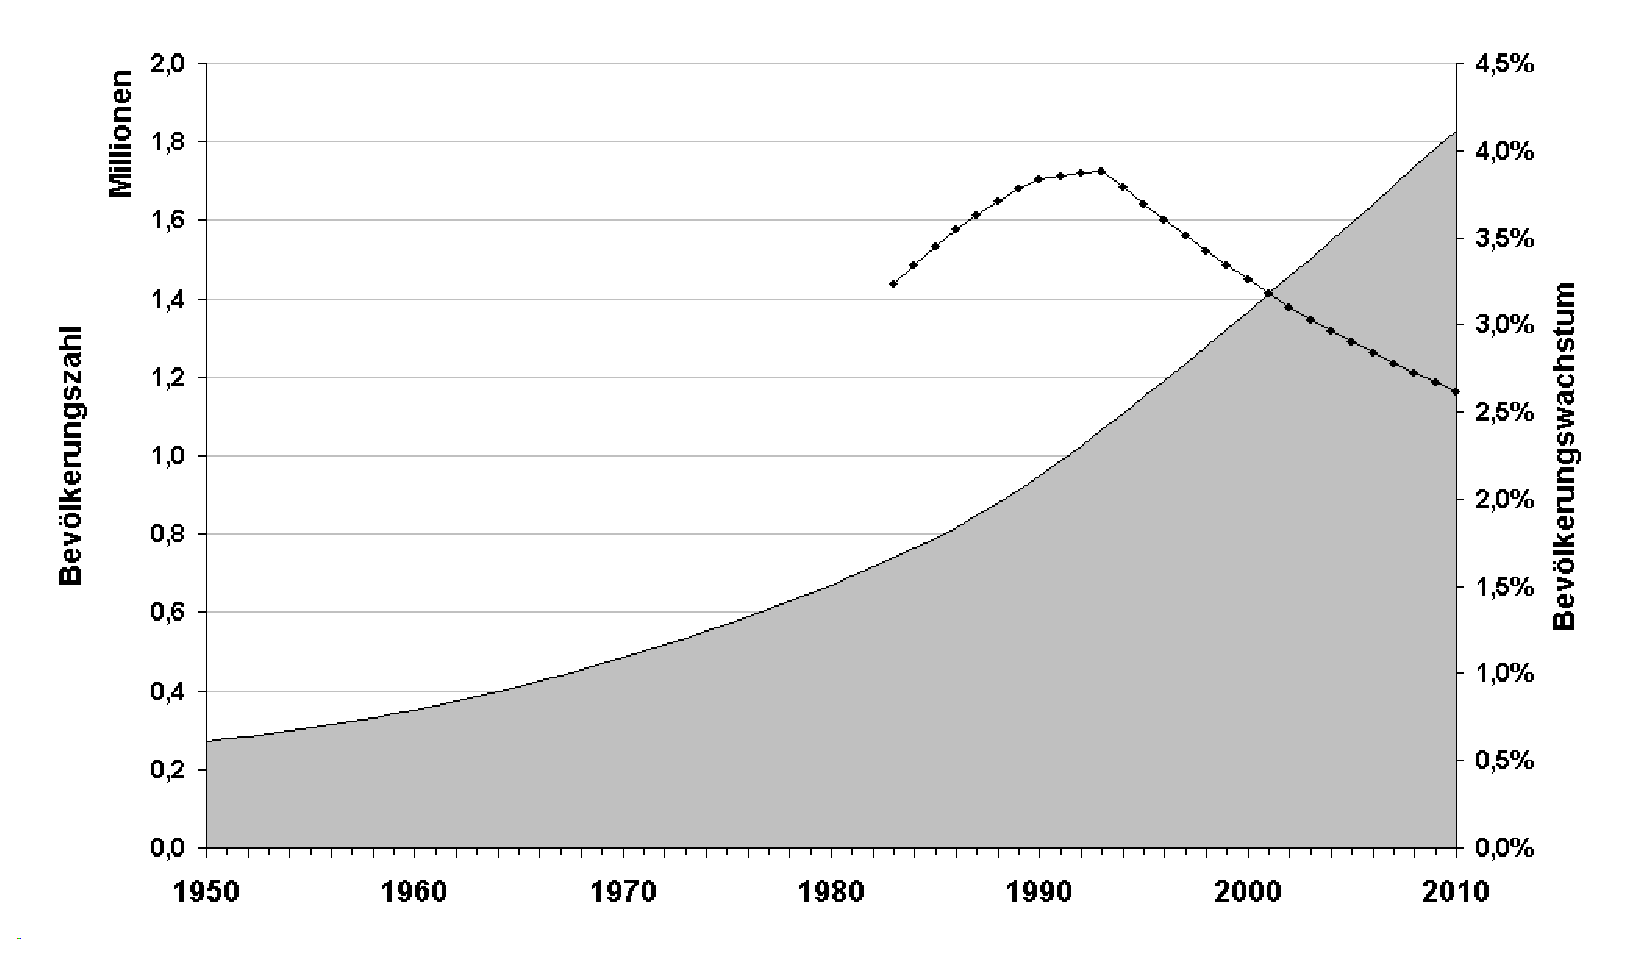
\includegraphics{../_database/Bilder/Bild36-1.eps}}

				
\subsection{Aufgabenstellung:}
\begin{enumerate}
	\item Um eine Prognose für die weitere Entwicklung der Bevölkerungszahl machen zu können, wird angenommen, dass die Wachstumsrate aus dem Jahr 2010 in den nachfolgenden Jahren konstant bleibt. Berechnen Sie näherungsweise mithilfe der Bevölkerungszahl des Jahres 2010, wie viele Jahre nach 2010 die Bevölkerungszahl von Gambia den Wert von 2,2 Mio. EinwohnerInnen unter dieser Annahme übersteigen wird!
	
 Betrachte den Graphen des Bevölkerungswachstums und entscheide, in welchen vier aufeinanderfolgenden Jahren von 1983 bis 2010 sich die Bevölkerungszahl am besten durch eine einzige Exponentialfunktion beschreiben lässt! Begründe deine Antwort!

\item Unter der Bevölkerungsdichte eines Landes versteht man die mittlere Anzahl der EinwohnerInnen pro $km^2$. In Österreich lag dieser Wert im Jahr 2010 bei 100 EinwohnerInnen pro $km^2$.

\fbox{A} Berechne für das Jahr 2010, um wie viel Prozent die Bevölkerungsdichte in Gambia  größer war als in Österreich!

Für den Zeitraum 1950-1990 lässt sich die Bevölkerungszahl $N(t)$ (in Mio. EinwohnerInnen) von Gambia annähernd durch die Gleichung 
$$N(t)= 0,2806\cdot e^{0,03\cdot t}$$
 beschreiben. Dabei wird $t$ in Jahren ab 1950 gemessen. Deute den Faktor 0,2806 im Hinblick auf die Bevölkerungszahl in Gambia und bestimme die Bevölkerungsdichte von Gambia für das Jahr 1973 nach diesem Modell!
						\end{enumerate}\leer
				
\antwort{
\begin{enumerate}
	\item \subsection{Lösungserwartung:} 
	
	Ansatz: $2,2=a\cdot b^t$, wobei der Wert für $a$ aus dem Intervall $[1,8; 1,85]$ und der Wert für $b$ aus dem Intervall $[1,025; 1,027]$ gewählt werden muss. Das Ergebnis für $t$ liegt demnach im Intervall $[6,5; 8,2]$.
 
 Für die Jahre 1990 bis 1993 lässt sich die Bevölkerungszahl am besten durch eine einzige Exponentialfunktion beschreiben, da die Prozentwerte des Bevölkerungswachstums annähernd konstant sind.
 
	 	
	\subsection{Lösungsschlüssel:}
	\begin{itemize}
		\item Ein Punkt für eine korrekte Berechnung.
		\item  Ein Punkt für eine (sinngemäß) korrekte Begründung. Die Lösung muss inhaltlich der Lösungserwartung entsprechen. Alle Vierjahresintervalle zwischen 1989 und 1994 sind (im Hinblick auf die Ablesegenauigkeit) zulässig.
	\end{itemize}
	
	\item \subsection{Lösungserwartung:}
		Ansatz: $\frac{a\cdot 1\,000\,000}{11\,000}$, wobei der Wert für $a$ aus dem Intervall $[1,8;1,85]$ gewählt werden muss. Das Ergebnis für die Bevölkerungsdichte liegt demnach im Intervall $[163,6; 168,2]$.
		
		Die Antwort auf die Frage, um wie viel Prozent die Bevölkerungsdichte in Gambia größer war als in Österreich, muss daher im Intervall $[63\,\%; 70\,\%]$ liegen.
		
		Der Faktor 0,2806 beschreibt die Bevölkerungszahl in Gambia im Jahr 1950 (in Mio. Einwohner/innen).
		
		$\frac{N(23)\cdot 1\,000\,000}{11\,000}\approx 50,86$
		
		Die Bevölkerungsdichte von Gambia für das Jahr 1973 liegt bei ca. 50,86 Einwohner/innen/km$^2$.
		
		
	\subsection{Lösungsschlüssel:}
	
\begin{itemize}
	\item Ein Augleichspunkt für eine korrekte Berechnung.
	\item  Ein Punkt für eine korrekte Berechnung und (sinngemäß korrekte Deutung der Bevölkerungsdichte von Gambia für das Jahr 1973. Lösungsintervall: $[50;51]$. Die Interpretation des Faktors muss sinngemäß der Lösungserwartung entsprechen.
\end{itemize}
\end{enumerate}}
		\end{langesbeispiel}